\tikzstyle{inner} = [circle, minimum size = 0.3cm, draw, inner sep = 0.1pt]

    
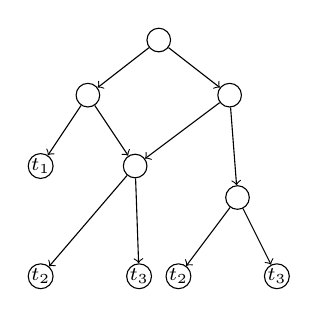
\begin{tikzpicture}
    \node[inner] (a) at (0, 0) {};
    \node[inner] (b) at (-0.9, -0.7) {};
    \node[inner] (c) at (0.9, -0.7) {};
    \node[inner] (d) at (-1.5, -1.6) {\scriptsize $t_1$};
    \node[inner] (e) at (-0.3, -1.6) {};
    \node[inner] (f) at (1, -2) {};
    \node[inner] (g) at (-1.5, -3) {\scriptsize $t_2$};
    \node[inner] (h) at (-0.25, -3) {\scriptsize $t_3$};
    \node[inner] (g2) at (1.5, -3) {\scriptsize $t_3$};
    \node[inner] (h2) at (0.25, -3) {\scriptsize $t_2$};
    
    \draw[->] (a) -- (b);
    \draw[->] (a) -- (c);
    \draw[->] (b) -- (d);
    \draw[->] (b) -- (e);
    \draw[->] (c) -- (e);
    \draw[->] (c) -- (f);
    \draw[->] (e) -- (g);
    \draw[->] (e) -- (h);
    \draw[->] (f) -- (g2);
    \draw[->] (f) -- (h2);
\end{tikzpicture}
